% load lecture note class
\documentclass{easyclass}
\usepackage[portuguese]{babel}
\usepackage{tcolorbox}
\usepackage{graphics}
\begin{document}
\begin{titlepage}
    \university{Universidade de Aveiro}
    \courseid{BD}
    \title{Apontamentos de BD}
    \author{Hugo Leal}
    \version{2021 Março}
    \instructor{Baseado nos slides de BD}
    \maketitle
\end{titlepage}

\tableofcontents
\clearpage

\section{Introdução aos sistemas de bases de dados}

\subsection{Conceito de Base de dados}
Uma base de dados é uma coleção organizada de dados que estão relacionados e que podem ser partilhados com múltiplas aplicações\\
\begin{tcolorbox}[
colframe=blue!25,
colback=blue!10,
coltitle=blue!20!black,  
fonttitle=\bfseries,
adjusted title=Evolução histórica]

\begin{itemize}
\item 50s - 60s   -   Processamento de dados isolados
\item 60s - 80s   -   Sistema de Gestão de Ficheiros
\item 80s - Hoje  -   Base de dados
\end{itemize}





\end{tcolorbox}

\subsection{Processamento de dados isolados}
No conceito de dados isolados cada aplicação gere os seus próprios dados, estes podem estar replicados, terem diferentes mas isto trás incoerências (problemas de "sincronismo")
\subsection{Sistema de Gestão de Ficheiros}
Os dados organizados e armazenados em ficheiros partilhados por várias aplicações.  Cada aplicação acede diretamente aos ficheiros e usa uma interface proprietária.  Isto trás problemas como:
\begin{itemize}
\item Problemas de acesso concorrente aos dados.
\item Problemas de integridade.
\item Problemas de segurança.
\end{itemize}
\section{Sistema de Gestão de base de dados}

\begin{tcolorbox}[
colframe=blue!25,
colback=blue!10,
coltitle=blue!20!black,  
fonttitle=\bfseries,
adjusted title=(DBMS) Database Management System]
É um sistema de uso geral que facilita o processo de definir, construir, manipular e partilhar bases de dados entre utilizadores e aplicações
\end{tcolorbox}

\subsection{Base de Dados}
Uma base de dados
\begin{itemize}
\item Definição (Defining)

\begin{itemize}
\item Especificação do tipo de dados, estruturas de dados e restrições
\end{itemize}

\item Construção (Constructing)
\begin{itemize}
\item Processo de armazenamento de dados
\end{itemize}

\item Manipulação (Manipulating)
\begin{itemize}
\item Envolve operações como a pesquisa e obtenção de dados
\end{itemize}

\item Partilha (Sharing)
\begin{itemize}
\item Acesso simultâneo aos dados por parte de vários utilizadores e programas
\end{itemize}

\end{itemize}

\subsection{SGDB - Características Gerais}
É uma entidade única que opera com a BD. O acesso à BD é sempre mediado pelo SGDB que contem uma interface de acesso que esconde os detalhes de armazenamento físico dos dados.  Isto trás uma elevada abstração ao nível aplicacional pois os dados estão integrados (nível lógico) numa mesma unidade de armazenamento. O SGDB suporta uma ou mais BD (Data Independence)
\subsection{SGDB - Vantagens}
\begin{itemize}
\item Independência entre programas e dados
\item Integridade dos dados,  o controlo de alteração de dados é realizado de acordo com as regras de integridade definidas
\item Consistência dos dados,  mesmo nos processos de transações e mesmo em falhas de software/hardware
\item Eficiência no acesso aos dados,  especialmente em cenários de manipulação de grandes quantidades de dados, por um ou mais utilizadores
\item Isolamento utilizadores, cada utilizador tem a "sensação" de ser o único
\item Melhor gestão do acesso concorrencial
\item Serviços de Segurança, como controlo de acessos/permissões e codificação de dados
\item Mecanismos de backup e recuperação de dados
\item Administração de dados, existe uma Disponibilidade de ferramentas desenvolvidas pelo fabricante e/ou terceiras entidades
\item Linguagem de desenho e manipulação de dados
\end{itemize}
É importante mencionar que muitas das vantagens anteriores são o requisito funcional de um SGBD
\subsection{SGBD - Utilizadores}
\begin{itemize}
    \item Utilizadores Finais
    
    \begin{itemize}
        \item aqueles que usam o sistema com determinada finalidade com recurso a ferramentas disponibilizadas pelo fabricante do sistema ou aplicações de terceiras entidades.
    \end{itemize}

    \item Programadores de Aplicações
    
    \begin{itemize}
        \item Desenvolvem aplicações que permitem que os utilizadores interajam com a base de dados. Podem utilizar várias linguagem de programação.
    \end{itemize}
    
    \item Administradores da Base de dados
    
    \begin{itemize}
        \item Tratam dos processos de gestão e manutenção da base de dados.
    \end{itemize}

\end{itemize}
\subsection{SGBD – Vista Simplificada}
    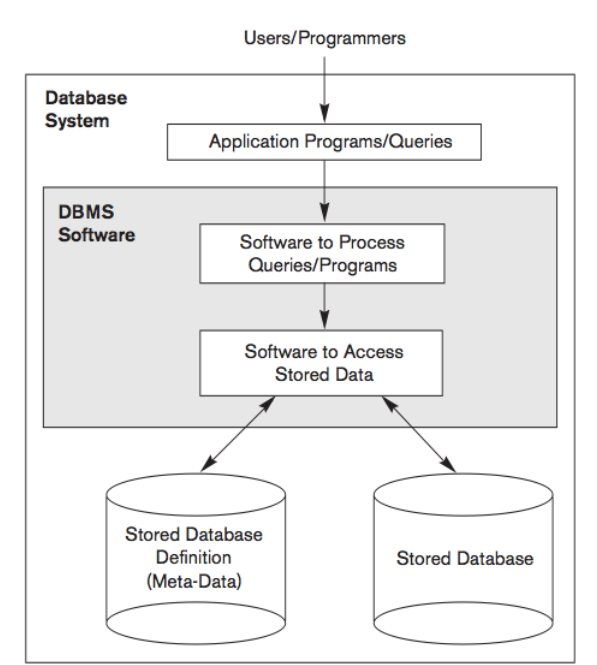
\includegraphics[width=10cm]{figures/1.png}

\subsection{SGBD – Dicionário de Dados}
O SGBD contém BD mas também informação relativa à descrição (definição) da própria estrutura da base de dados, incluindo as restrições (um dicionário)
Este dicionário contem:
\begin{itemize}
    \item Descritores de objetos da base de dados (tabelas, utilizadores, regras, vistas, indexes, etc)
    \item Informação sobre dados em uso e por quem (locks).
    \item Schemas e mappings
\end{itemize}
\subsection{SGBD – Arquitetura ANSI/SPARC}
Contem tres níveis: Externo; Comceptual; Interno
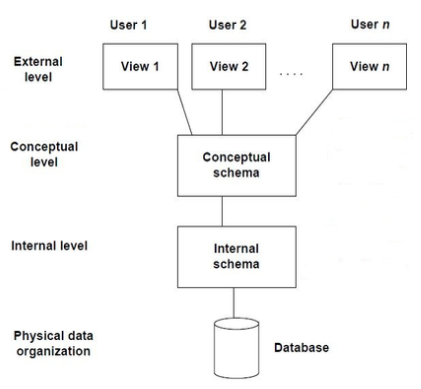
\includegraphics[width=10cm]{figures/2.png}
\subsubsection{Nível Interno}
Pode ser lida como a implementação física da BD. Contem a estrutura dos registos em disco - files, pages, blocks e, indexes e ordenação dos registos.\\
É do domínio dos programadores de sistemas de BD\\
Exemplo de um esquema: 
\begin{verbatim}
    RECORD FUNCIONARIO
        LENGTH=44
    HEADER: BYTE(5)
        OFFSET=0
    NOME: BYTE(25)
        OFFSET=5
    SALARIO: FULLWORD
        OFFSET=30
    DEPARTAMENTO: BYTE(10)
        OFFSET=34
\end{verbatim}
\subsubsection{Nível Conceptual}
O esquema Conceptual, descreve a estrutura da base de dados para os utilizadores. Descreve entidades, tipo de dados, relações, operações, restrições, etc e utiliza (tipicamente) um modelo de dados para descrição do esquema conceptual\\
Oculta detalhes de implementação física(abstração)
É do domínio do administrador da BD e do programador de aplicações\\
Exemplo de esquema:\\
\begin{verbatim}
    CREATE TABLE FUNCIONARIO
      (Nome VARCHAR(25), 
    Salario REAL, Dept_Nome VARCHAR(10))
\end{verbatim}
\subsubsection{Nível Externo}

%\bibliography{bibfile}
\end{document}